\documentclass[tikz]{standalone}
\usetikzlibrary{positioning}
\usepackage{amsmath}
\usepackage{mathrsfs}

\newcommand{\cat}[1]{\mathscr{#1}}
\newcommand{\obj}[1]{\lowercase{#1}}
\newcommand{\objs}[1]{#1}
\newcommand{\mrp}[3]{{#1}:{#2}\to{#3}}
\newcommand{\mrps}[3]{#1(#2,#3)}
\newcommand{\id}[1]{\mathrm{id}_{#1}}
\newcommand{\op}[1]{{#1}^{\mathrm{op}}}
\newcommand{\set}{\mathbf{Set}}
\newcommand{\Top}{\mathsf{Top}}
\newcommand{\blat}{\mathsf{BLat}}
\newcommand{\stone}{\mathsf{Stone}}
\DeclareMathOperator{\dom}{dom}
\DeclareMathOperator{\cod}{cod}
\DeclareMathOperator{\colim}{Colim}
\DeclareMathOperator{\lan}{Lan}
\DeclareMathOperator{\ran}{Ran}
\DeclareMathOperator{\cone}{Cone}
\DeclareMathOperator{\cocone}{Cocone}


\begin{document}
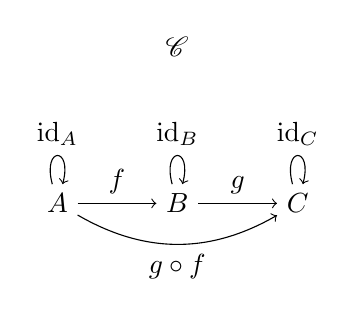
\begin{tikzpicture}
	\node (A) {$A$};
	\node [right=1cm of A] (B) {$B$};
	\node [right=1cm of B] (C) {$C$};
	\node [above=1.5cm of B] (catc) {$\cat{C}$};
	\draw [->] (A) to [edge label=$f$] (B);
	\draw [->] (B) to [edge label=$g$] (C);
	\draw [->, bend right] (A) to node [below] {$g\circ f$} (C);
	\draw [->, loop above] (A) to node [above] {$\id{A}$} (A);
	\draw [->, loop above] (B) to node [above] {$\id{B}$} (B);
	\draw [->, loop above] (C) to node [above] {$\id{C}$} (C);
\end{tikzpicture}
\end{document}
